\documentclass[man,floatsintext]{apa6}
\usepackage{lmodern}
\usepackage{amssymb,amsmath}
\usepackage{ifxetex,ifluatex}
\usepackage{fixltx2e} % provides \textsubscript
\ifnum 0\ifxetex 1\fi\ifluatex 1\fi=0 % if pdftex
  \usepackage[T1]{fontenc}
  \usepackage[utf8]{inputenc}
\else % if luatex or xelatex
  \ifxetex
    \usepackage{mathspec}
  \else
    \usepackage{fontspec}
  \fi
  \defaultfontfeatures{Ligatures=TeX,Scale=MatchLowercase}
\fi
% use upquote if available, for straight quotes in verbatim environments
\IfFileExists{upquote.sty}{\usepackage{upquote}}{}
% use microtype if available
\IfFileExists{microtype.sty}{%
\usepackage{microtype}
\UseMicrotypeSet[protrusion]{basicmath} % disable protrusion for tt fonts
}{}
\usepackage{hyperref}
\hypersetup{unicode=true,
            pdftitle={Cognitive correlates of mental health in adolescence: A network analysis approach},
            pdfauthor={Sam Parsons, Annabel Songco, Charlotte Booth, \& Elaine Fox},
            pdfkeywords={keywords},
            pdfborder={0 0 0},
            breaklinks=true}
\urlstyle{same}  % don't use monospace font for urls
\usepackage{graphicx,grffile}
\makeatletter
\def\maxwidth{\ifdim\Gin@nat@width>\linewidth\linewidth\else\Gin@nat@width\fi}
\def\maxheight{\ifdim\Gin@nat@height>\textheight\textheight\else\Gin@nat@height\fi}
\makeatother
% Scale images if necessary, so that they will not overflow the page
% margins by default, and it is still possible to overwrite the defaults
% using explicit options in \includegraphics[width, height, ...]{}
\setkeys{Gin}{width=\maxwidth,height=\maxheight,keepaspectratio}
\IfFileExists{parskip.sty}{%
\usepackage{parskip}
}{% else
\setlength{\parindent}{0pt}
\setlength{\parskip}{6pt plus 2pt minus 1pt}
}
\setlength{\emergencystretch}{3em}  % prevent overfull lines
\providecommand{\tightlist}{%
  \setlength{\itemsep}{0pt}\setlength{\parskip}{0pt}}
\setcounter{secnumdepth}{0}
% Redefines (sub)paragraphs to behave more like sections
\ifx\paragraph\undefined\else
\let\oldparagraph\paragraph
\renewcommand{\paragraph}[1]{\oldparagraph{#1}\mbox{}}
\fi
\ifx\subparagraph\undefined\else
\let\oldsubparagraph\subparagraph
\renewcommand{\subparagraph}[1]{\oldsubparagraph{#1}\mbox{}}
\fi

%%% Use protect on footnotes to avoid problems with footnotes in titles
\let\rmarkdownfootnote\footnote%
\def\footnote{\protect\rmarkdownfootnote}


  \title{Cognitive correlates of mental health in adolescence: A network analysis
approach}
    \author{Sam Parsons\textsuperscript{1}, Annabel Songco\textsuperscript{1},
Charlotte Booth\textsuperscript{1}, \& Elaine Fox\textsuperscript{1}}
    \date{}
  
\shorttitle{Combined Cognitive Bias Hypothesis Network}
\affiliation{
\vspace{0.5cm}
\textsuperscript{1} University of Oxford}
\keywords{keywords\newline\indent Word count: X}
\usepackage{csquotes}
\usepackage{upgreek}
\captionsetup{font=singlespacing,justification=justified}

\usepackage{longtable}
\usepackage{lscape}
\usepackage{multirow}
\usepackage{tabularx}
\usepackage[flushleft]{threeparttable}
\usepackage{threeparttablex}

\newenvironment{lltable}{\begin{landscape}\begin{center}\begin{ThreePartTable}}{\end{ThreePartTable}\end{center}\end{landscape}}

\makeatletter
\newcommand\LastLTentrywidth{1em}
\newlength\longtablewidth
\setlength{\longtablewidth}{1in}
\newcommand{\getlongtablewidth}{\begingroup \ifcsname LT@\roman{LT@tables}\endcsname \global\longtablewidth=0pt \renewcommand{\LT@entry}[2]{\global\advance\longtablewidth by ##2\relax\gdef\LastLTentrywidth{##2}}\@nameuse{LT@\roman{LT@tables}} \fi \endgroup}


\usepackage{lineno}

\linenumbers
\usepackage{float}
\floatplacement{figure}{H}
\raggedbottom

\authornote{Add complete departmental affiliations for each
author here. Each new line herein must be indented, like this line.

Enter author note here.

Correspondence concerning this article should be addressed to Sam
Parsons, Postal address. E-mail:
\href{mailto:sam.parsons@psy.ox.ac.uk}{\nolinkurl{sam.parsons@psy.ox.ac.uk}}}

\abstract{
This is my abstract


}

\begin{document}
\maketitle

The introduction section will not need much of an update. There will
need to be some revisions based on my updated understanding, as well as
reviewer feedback, but we should be in good standing here.

\section{Methods}\label{methods}

The methods section will not need to be massively updated.

\subsection{Participants}\label{participants}

\subsection{Measures}\label{measures}

\subsubsection{Mental Health Continuum}\label{mental-health-continuum}

\subsubsection{Attention Bias}\label{attention-bias}

\subsubsection{Interpretation Bias}\label{interpretation-bias}

\subsubsection{Memory Bias}\label{memory-bias}

\subsection{Procedure}\label{procedure}

\subsection{Data analysis and network
visualisation}\label{data-analysis-and-network-visualisation}

\subsubsection{Gaussian Graphical Model}\label{gaussian-graphical-model}

\subsubsection{Mixed Graphical Model and moderated network
analysis}\label{mixed-graphical-model-and-moderated-network-analysis}

\subsubsection{network centrality
indices}\label{network-centrality-indices}

\subsubsection{Network stability}\label{network-stability}

\begin{verbatim}
[1] 40.77902
\end{verbatim}

\begin{verbatim}
[1] 12.59799
\end{verbatim}

\begin{verbatim}
33% 66% 
 37  47 
\end{verbatim}

\begin{figure}
\centering
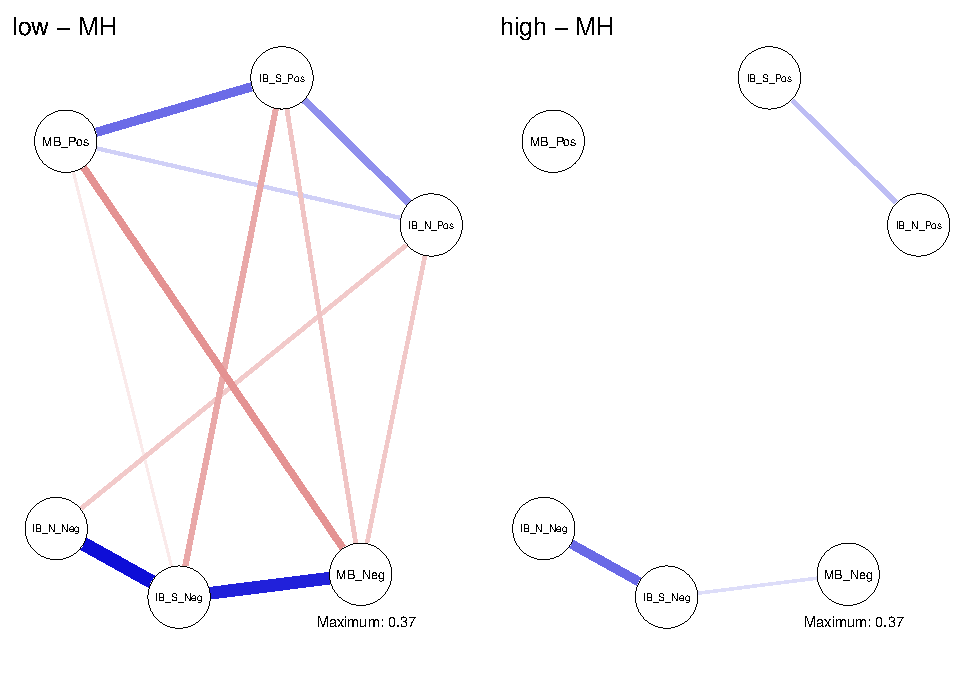
\includegraphics{script_files/figure-latex/glasso networks-1.pdf}
\caption{}
\end{figure}

\begin{verbatim}
[1] 1.801493
\end{verbatim}

\begin{verbatim}
[1] 0.6046656
\end{verbatim}

\begin{verbatim}
[1] 0.3676674
\end{verbatim}

\begin{figure}
\centering
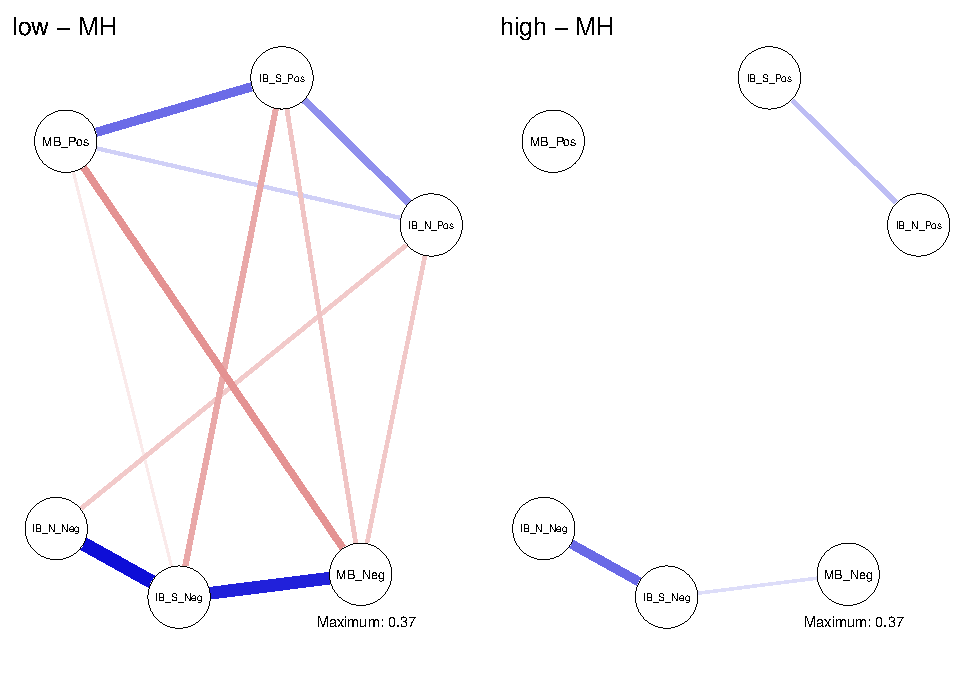
\includegraphics{script_files/figure-latex/glasso networks-2.pdf}
\caption{}
\end{figure}

\subsubsection{network comparisons}\label{network-comparisons}

results from the NCT show that the low group differs from the high group
(strength p = 0.00 and biggest edge difference p = 0.02) and the mid
group perhaps differed (global strength may not survive multiple
comparisons though, and max diff was n.s different. ). The mid and high
groups do not differ.

\subsubsection{mgm}\label{mgm}

we then explored this in a more robust way using mgm\ldots{}

\paragraph{im mainly curious what this
is}\label{im-mainly-curious-what-this-is}

seriously what does the four hashes mean???

\begin{figure}
\centering
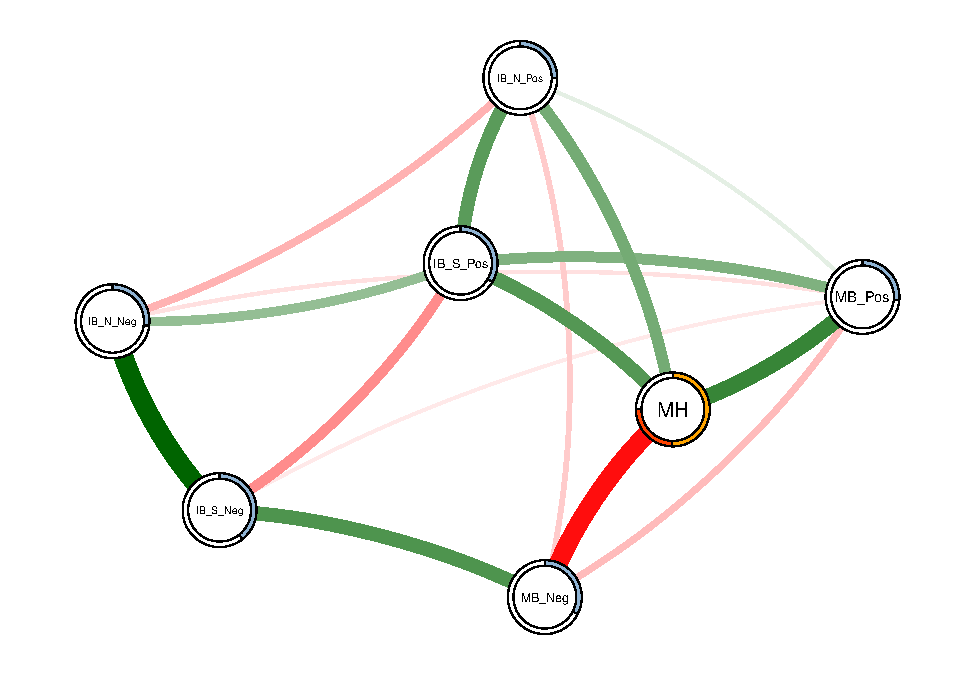
\includegraphics{script_files/figure-latex/mgm-1.pdf}
\caption{}
\end{figure}

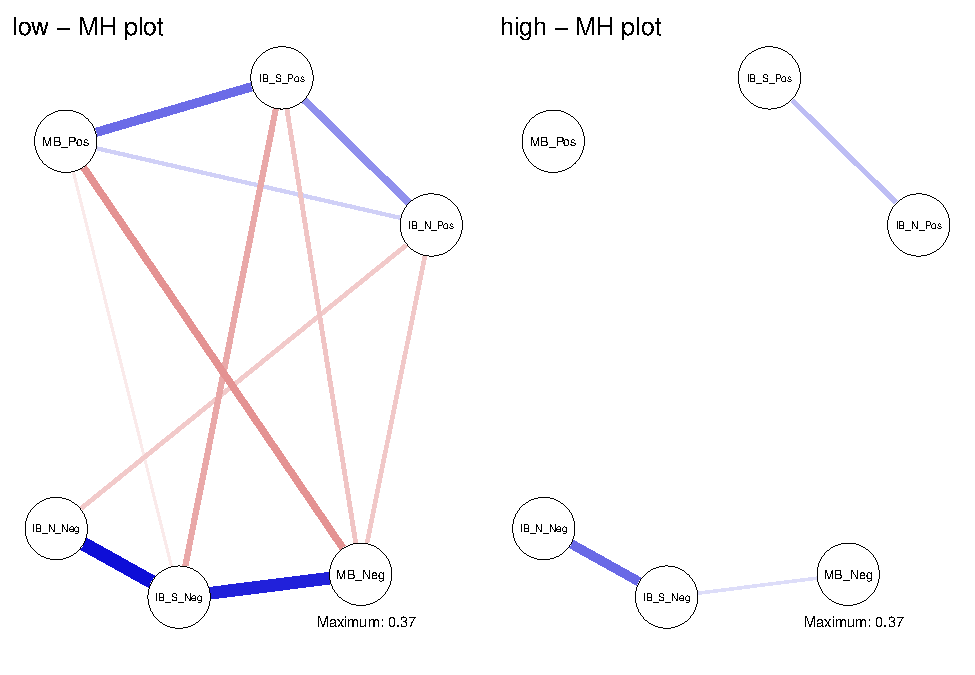
\includegraphics{script_files/figure-latex/unnamed-chunk-1-1.pdf}
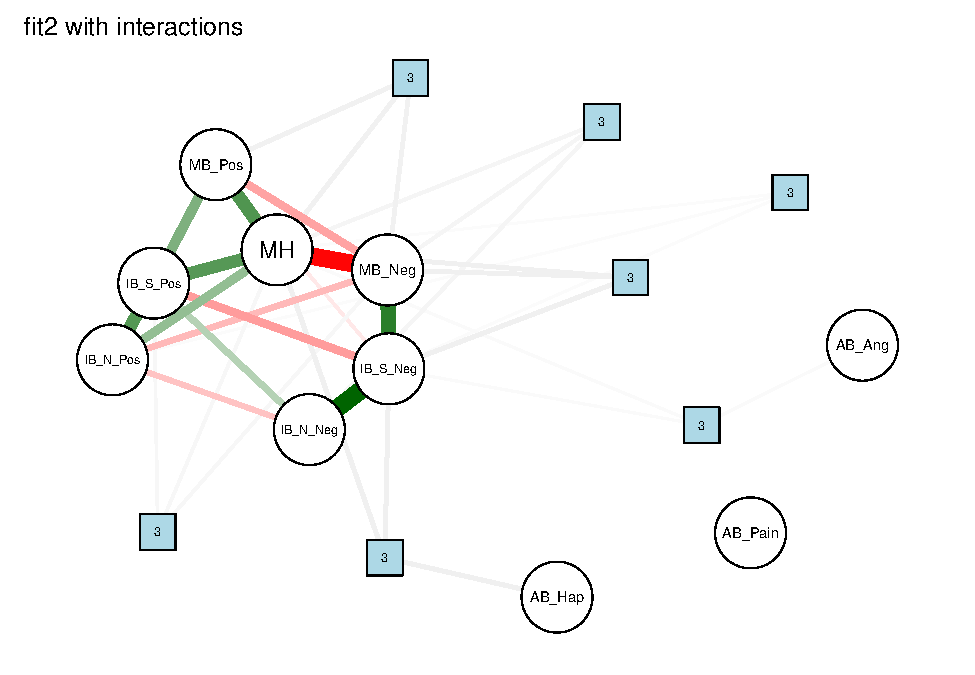
\includegraphics{script_files/figure-latex/unnamed-chunk-1-2.pdf}
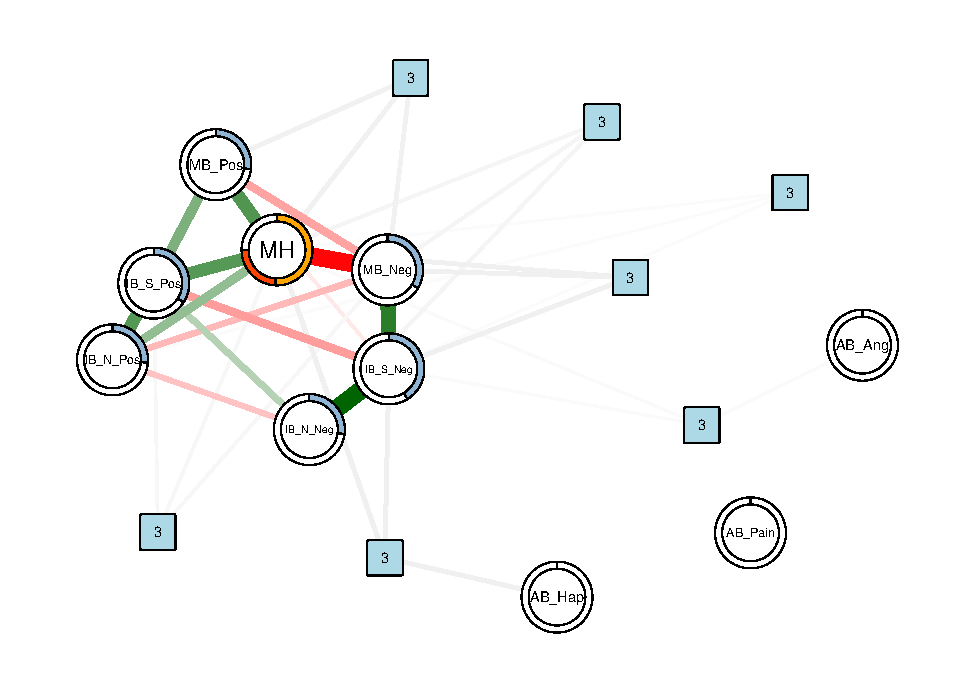
\includegraphics{script_files/figure-latex/unnamed-chunk-1-3.pdf}

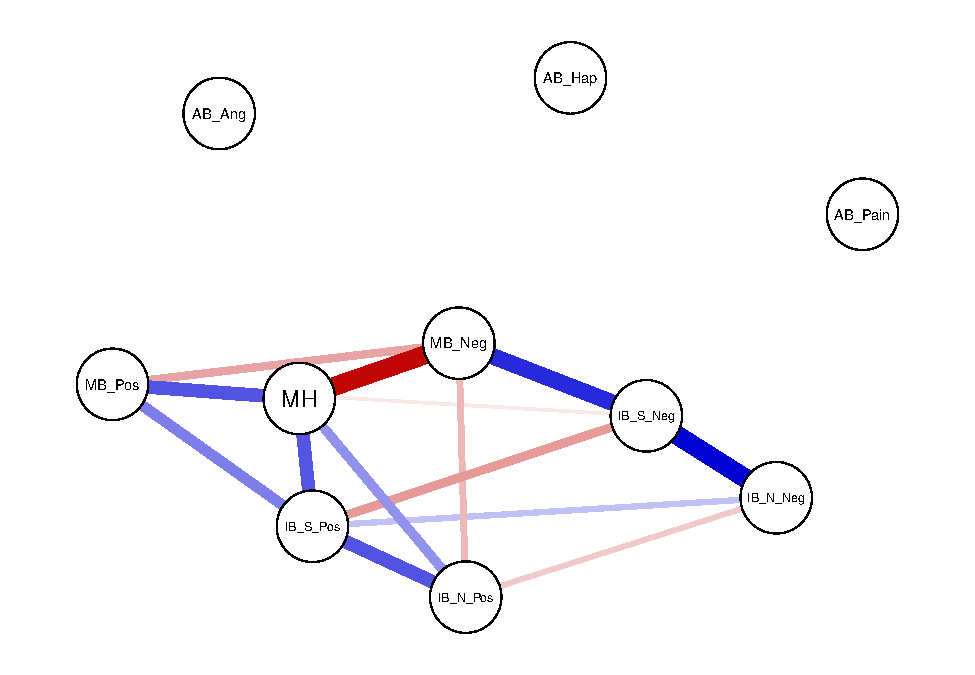
\includegraphics{script_files/figure-latex/stability-1.pdf}
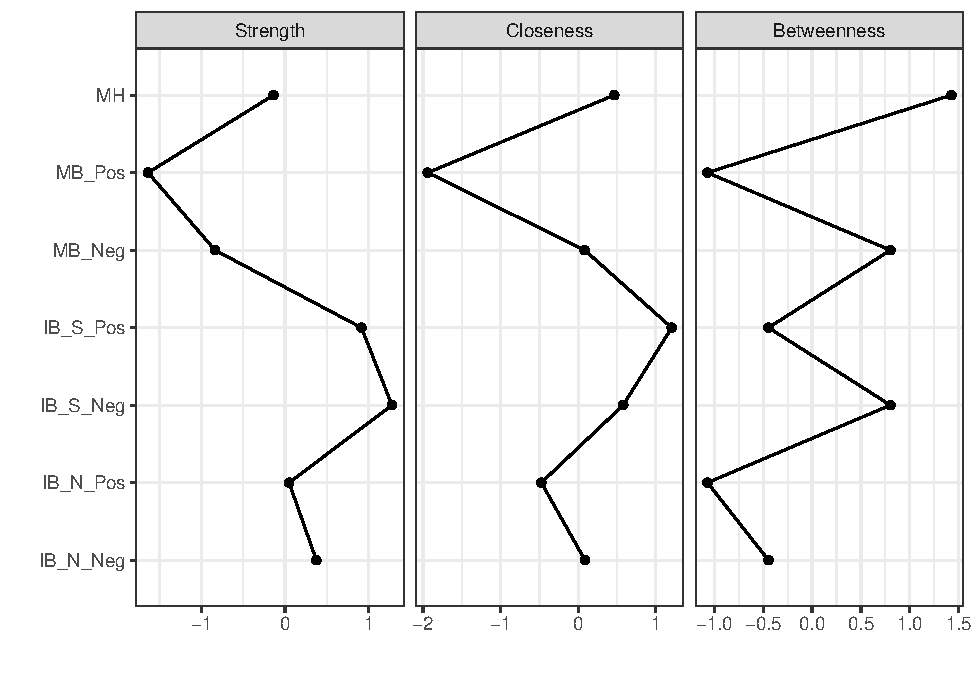
\includegraphics{script_files/figure-latex/stability-2.pdf}

\begin{verbatim}

  |                                                                       
  |                                                                 |   0%
  |                                                                       
  |------                                                           |  10%
  |                                                                       
  |-------------                                                    |  20%
  |                                                                       
  |--------------------                                             |  30%
  |                                                                       
  |--------------------------                                       |  40%
  |                                                                       
  |--------------------------------                                 |  50%
  |                                                                       
  |---------------------------------------                          |  60%
  |                                                                       
  |----------------------------------------------                   |  70%
  |                                                                       
  |----------------------------------------------------             |  80%
  |                                                                       
  |----------------------------------------------------------       |  90%
  |                                                                       
  |-----------------------------------------------------------------| 100%
Note that the sign of parameter estimates is stored separately; see ?mgm
\end{verbatim}

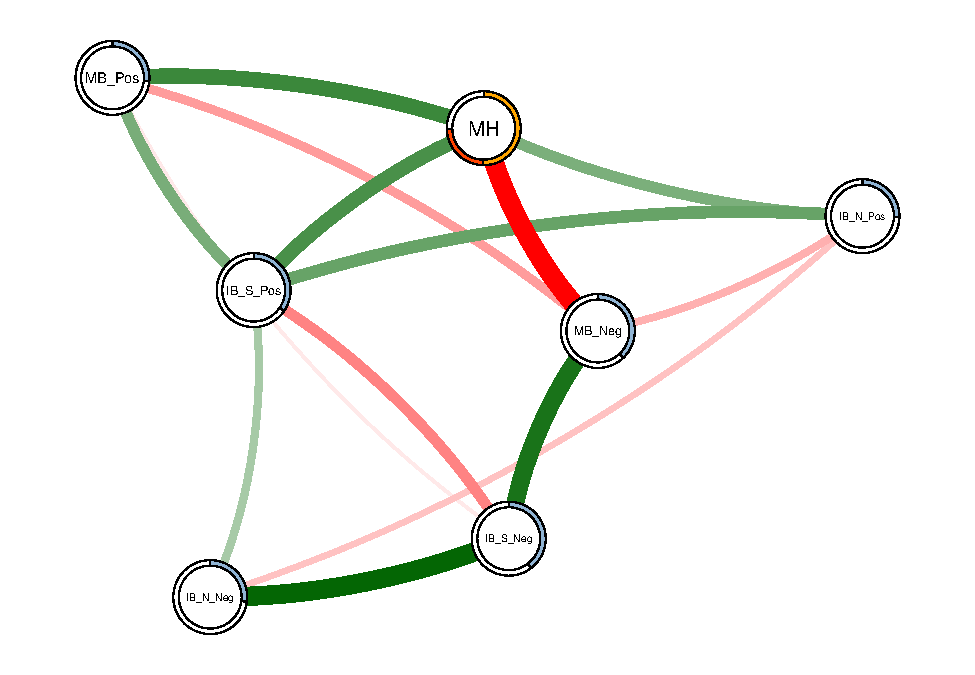
\includegraphics{script_files/figure-latex/unnamed-chunk-2-1.pdf}
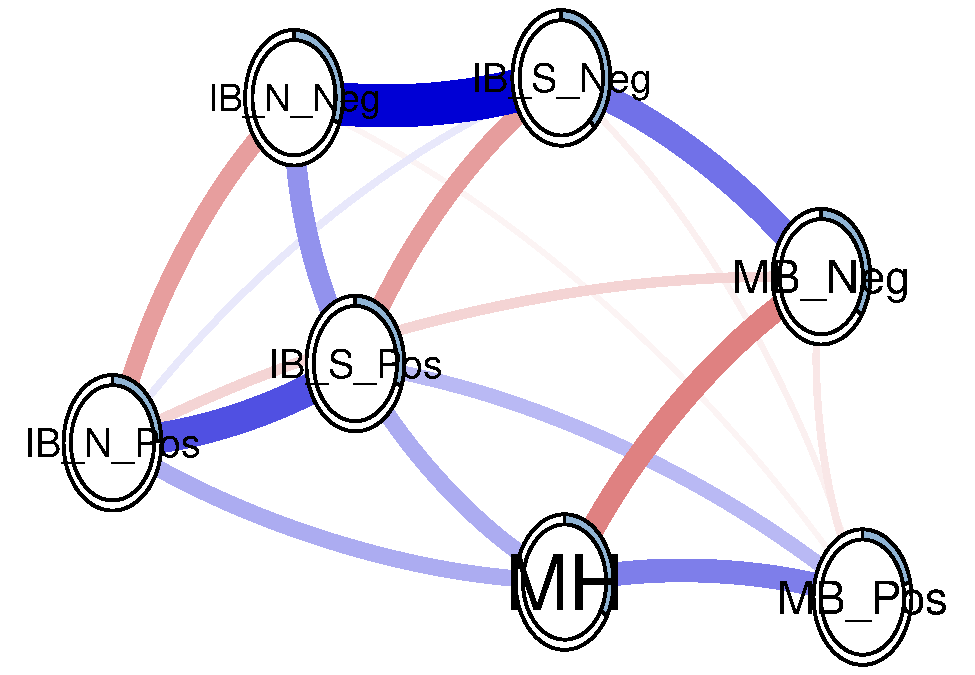
\includegraphics{script_files/figure-latex/unnamed-chunk-2-2.pdf}

\section{Results}\label{results}

\subsection{glasso networks}\label{glasso-networks}

\subsection{moderated networks}\label{moderated-networks}

\section{Discussion}\label{discussion}

\newpage

\section{References}\label{references}

\begingroup
\setlength{\parindent}{-0.5in} \setlength{\leftskip}{0.5in}

\hypertarget{refs}{}

\endgroup


\end{document}
